\documentclass[11pt,notes=hide,aspectratio=169,mathserif]{beamer}

% PACKAGES
\usepackage{graphics}  % Support for images/figures
\usepackage{graphicx}  % Includes the \resizebox command
\usepackage{url}	   % Includes \urldef and \url commands
\usepackage{natbib}
\usepackage{bibentry}  % Includes the \nobibliography command
\usepackage{verbatim}  %Supports comments
\usepackage{booktabs} %Supports \toprule, \bottomrule, etc in tables
\usepackage{threeparttable} %Supports tablenotes in tables
\usepackage{adjustbox} %Supports fitting tables to a maximum size
\usepackage{array} %Supports ragged-right table columns
\usepackage{etoolbox}  %Supports toggle commands
\usepackage{bm}	%Supports bold math \bm
\usepackage{enumitem}

% Citation styling - smaller and light grey
\definecolor{citegray}{gray}{0.5}

% Save original citation commands
\let\origcitep\citep
\let\origcite\cite
\let\origcitet\citet

% Redefine with smaller size and grey color
\renewcommand{\citep}[2][]{\begingroup\scriptsize\color{citegray}\origcitep[#1]{#2}\endgroup}
\renewcommand{\cite}[2][]{\begingroup\scriptsize\color{citegray}\origcite[#1]{#2}\endgroup}
\renewcommand{\citet}[2][]{\begingroup\scriptsize\color{citegray}\origcitet[#1]{#2}\endgroup}

% PACKAGES (that should already be included by your LyX document settings)
\usepackage{amsfonts}  % Lots of stuff, including \mathbb
\usepackage{amsmath}   % Standard math package
\usepackage{amsthm}    % Includes the comment functions
\usepackage{dsfont}

% CUSTOM DEFINITIONS
\def\newblock{} %Get beamer to cooperate with BibTeX

\setlist[itemize,1]{label=\usebeamertemplate{itemize item}}
\setlist[itemize,2]{label=\usebeamertemplate{itemize subitem}}
\setlist[itemize,3]{label=\usebeamertemplate{itemize subsubitem}}
\setlist[enumerate,1]{label=\insertenumlabel.}
\setlist[enumerate,2]{label=\insertsubenumlabel.}
\setlist[enumerate,3]{label=\insertsubsubenumlabel.}

% NUMBERS FROM THE ANALYSIS
\input{../tasks/audits/audit_scale_shape_splitting/output/figure_guide_values.tex}
\input{../tasks/estimate_notch_model/output/model_values.tex}

% IDENTIFYING INFORMATION
\title[Housing Regulation]{The Cost of Housing Regulation: Evidence from Bunching in New York City}
\author[Jacob Herbstman]{Jacob Herbstman (University of Chicago)}
\date{October 2026}

% THEMATIC OPTIONS
\setbeamercovered{transparent}
\usetheme{metropolis}
\linespread{1.0}
\usecolortheme{default}
\beamertemplatenavigationsymbolsempty
\setbeamertemplate{footline}[frame number]{}

% BACKUP SLIDE NUMBERING
\usepackage{appendixnumberbeamer}

\begin{document}

%---------------------------------------------------------------------
\begin{frame}[plain]
\titlepage
\end{frame}
%---------------------------------------------------------------------

% PART 1: MOTIVATION
\begin{frame}
    \frametitle{485-x Makes 100 Units a Threshold}
    \begin{itemize}[itemsep=0.5em]
        \item New York City's main tax incentive for new rental housing, replacing 421-a in 2024
        \item Rental sites with 100 or more units face stricter affordability rules and a construction wage floor
        \item Sites can avoid the threshold by building fewer units or by dividing a project into smaller parts
    \end{itemize}
\end{frame}

\begin{frame}
    \frametitle{Developers Are Proposing 99-Unit Buildings}
    \begin{columns}[c,onlytextwidth]
        \begin{column}{0.52\textwidth}
            \centering
            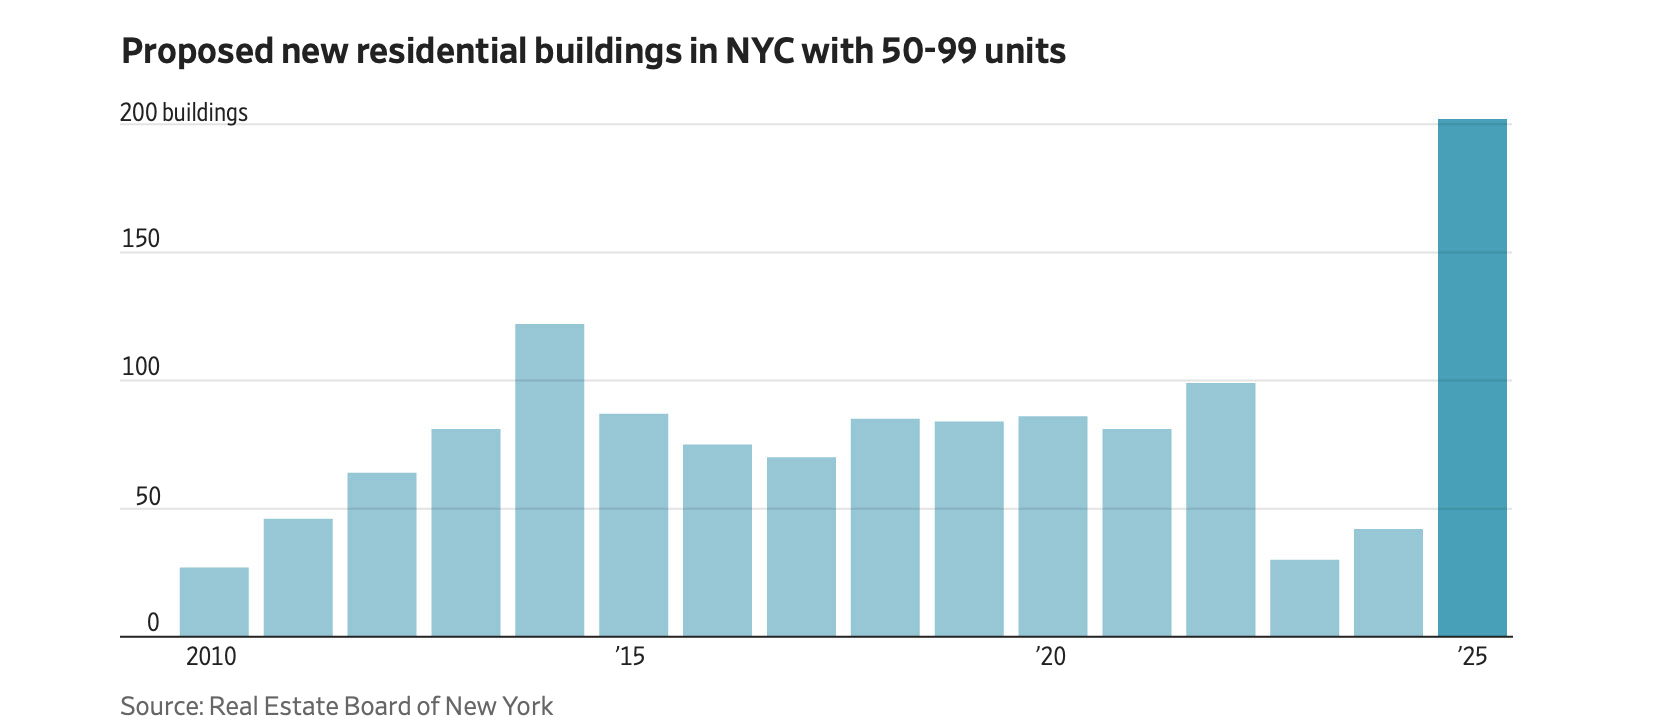
\includegraphics[width=\linewidth]{images/wsj_50_99_unit_buildings.png}
            \par\vspace{0.8em}
            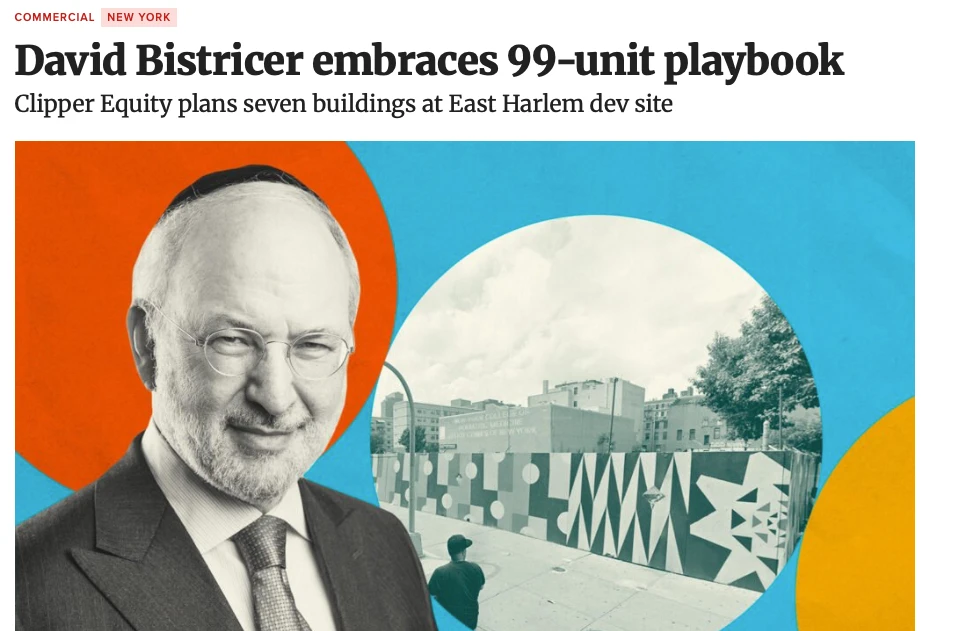
\includegraphics[width=\linewidth,height=0.4\textheight,keepaspectratio]{images/real_deal_bistricer_99_unit_playbook.png}
        \end{column}
        \begin{column}{0.45\textwidth}
            \centering
            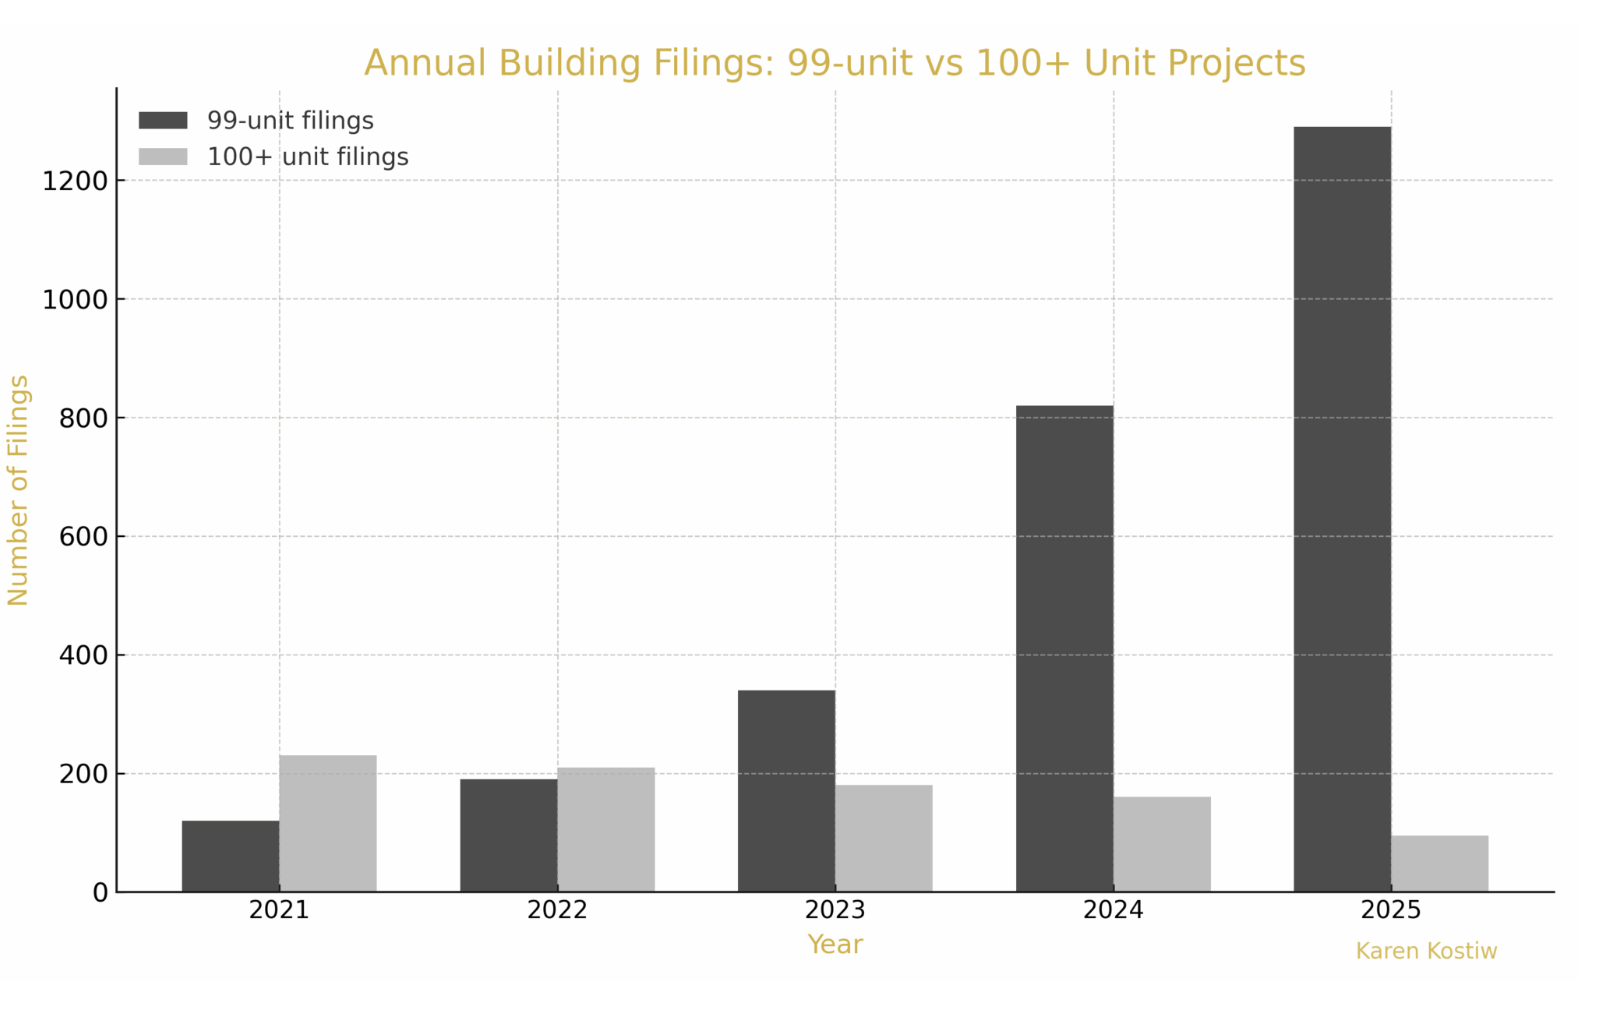
\includegraphics[width=\linewidth]{images/kostiw_99_unit_filings.png}
        \end{column}
    \end{columns}
\end{frame}

\begin{frame}
    \frametitle{Fewer Units or a Different Project Design?}
    \begin{itemize}[itemsep=0.5em]
        \item A 110-unit project cut to 99 loses 11 apartments
        \item The same project split into two buildings of 55 loses none
        \item A 210-unit project built as 99 + 99 loses 12
    \end{itemize}
    \vspace{0.5em}
    The housing cost of the threshold depends on which response developers choose.
\end{frame}

\begin{frame}
    \frametitle{This Paper}
    \begin{itemize}[itemsep=0.5em]
        \item Link new-building filings into parent projects, before and after 485-x
        \item Recent projects bunch at 99 units and at 99 + 99
        \item The share of projects split into several buildings rises
        \item A model of project size and splitting implies about \MainUnitsLost{} fewer proposed units among recent projects
    \end{itemize}
\end{frame}


% PART 2: RELATED LITERATURE
\begin{frame}
    \frametitle{Related Literature}

    \textbf{Bunching at kinks and notches}
    \begin{itemize}[itemsep=2pt, topsep=3pt]
        \item Taxes and firms \cite{saez2010,chetty2011,klevenwaseem2013,kleven2016,garicano2016}
        \item Housing transactions and building heights \cite{kopczukmunroe2015,bestkleven2018,brueckner2024}
    \end{itemize}

    \vspace{2pt}
    \textbf{Housing regulation and tax incentives}
    \begin{itemize}[itemsep=2pt, topsep=3pt]
        \item Regulation and housing supply \cite{glaeser2005}
        \item Inclusionary housing and 421-a \cite{schuetz2011,soltas2024}
    \end{itemize}

    \vspace{2pt}
    \textbf{Costs revealed by choices}
    \begin{itemize}[itemsep=2pt, topsep=3pt]
        \item Prices, entry and replacement \cite{rust1987,bresnahanreiss1991,blp1995}
    \end{itemize}
\end{frame}


% PART 3: DATA
\begin{frame}
    \frametitle{Data}
    \begin{itemize}[itemsep=0.5em]
        \item New-building filings: DCP Housing Database (2019--2022) and DOB NOW (2025--2026)
        \item Parcels: archived MapPLUTO releases from before each filing
        \item Tenure and program: HPD 485-x registrations and Attorney General condominium plans
    \end{itemize}
\end{frame}

\begin{frame}
    \frametitle{From Filings to Parent Projects}
    \begin{itemize}[itemsep=0.5em]
        \item Related filings within a year are linked into one parent: same site, same owner nearby, or explicit references
        \item The same rules apply in both periods
        \item Sample: rental parents of at least 50 units, \CalibrationHistoricalParents{} from 2019--2022 and \CalibrationPostParents{} from January 2025 to July 2026
        \item Historical parents are reweighted to match recent sites on zoning and borough
    \end{itemize}
\end{frame}


% PART 4: EMPIRICAL RESULTS
\begin{frame}
    \frametitle{Project Sizes Before and After 485-x}
    \centering
    \only<1>{\includegraphics[width=\textwidth,height=0.82\textheight,keepaspectratio]{../tasks/presentation_figures/output/pdf/parent_bunching_2019_2022.pdf}}%
    \only<2>{\includegraphics[width=\textwidth,height=0.82\textheight,keepaspectratio]{../tasks/presentation_figures/output/pdf/parent_bunching_both_periods.pdf}}
\end{frame}

\begin{frame}
    \frametitle{Excess Mass at 99 and 198, a Shortfall Above 100}
    \centering
    \begin{tabular}{@{}lrrrr@{}}
        \toprule
        Parent units & 2019--2022 (\%) & 2025--2026 (\%) & Difference (pp) & 95\% interval \\
        \midrule
        99 & \HistoricalShareNinetyNine & \PostShareNinetyNine & \ExcessNinetyNine & [\ExcessNinetyNineLower, \ExcessNinetyNineUpper] \\
        100--149 & \HistoricalShareOneHundredOneFortyNine & \PostShareOneHundredOneFortyNine & $-$\DeficitOneHundredOneFortyNine & [$-$\DeficitOneHundredOneFortyNineUpper, $-$\DeficitOneHundredOneFortyNineLower] \\
        198 & \HistoricalShareOneNinetyEight & \PostShareOneNinetyEight & \ExcessOneNinetyEight & [\ExcessOneNinetyEightLower, \ExcessOneNinetyEightUpper] \\
        \bottomrule
    \end{tabular}
    \par\vspace{0.8em}
    {\footnotesize Shares of parents of at least 50 units; historical shares reweighted. Every recent 198-unit parent is two 99-unit buildings.}
\end{frame}

\begin{frame}
    \frametitle{Many 99-Unit Buildings Belong to Larger Projects}
    \centering
    \includegraphics[width=\textwidth,height=0.82\textheight,keepaspectratio]{../tasks/plot_bunching/output/pdf/parents_with_99_unit_constituents.pdf}
\end{frame}

\begin{frame}
    \frametitle{More Projects Are Split Into Several Buildings}
    \centering
    \includegraphics[width=\textwidth,height=0.82\textheight,keepaspectratio]{../tasks/plot_bunching/output/pdf/splitting_by_year.pdf}
\end{frame}


% PART 5: MODEL
\begin{frame}
    \frametitle{Without the Policy}
    \begin{itemize}[itemsep=0.5em]
        \item Developer $i$ prefers to build $x_i$ units in $J_i^0$ buildings
        \item Building $m$ units instead costs
        \[
          \Big(\frac{m-x_i}{99}\Big)^2,
        \]
        relative to the cost of building 99 units
        \item Without the policy, every developer builds $x_i$ in $J_i^0$ buildings
        \item 2019--2022 projects tell us $x_i$ and $J_i^0$
    \end{itemize}
\end{frame}

\begin{frame}
    \frametitle{Adding the Notch at 100 Units}
    \begin{itemize}[itemsep=0.5em]
        \item A building of 100 units or more costs an extra $b_i\kappa$
        \item With one building, the developer solves
        \[
          \min_m\; \Big(\frac{m-x_i}{99}\Big)^2 + b_i\kappa\,\mathbf{1}\{m\ge100\}
        \]
        \item Shrink to 99 if $x_i < 99\big(1+\sqrt{b_i\kappa}\big)$; otherwise build $x_i$ and pay
        \item $b_i$ varies across developers: lognormal with median 1 and spread $s$
        \item Why it varies: the burden depends on what a developer already pays, such as how far its usual wages are below the required wage (wage data to come)
    \end{itemize}
\end{frame}

\begin{frame}
    \frametitle{Adding the Choice to Split}
    The developer chooses total units $m$ and buildings $J$, with $m=n_1+\dots+n_J$:
    \[
      \min_{m,J}\; \Big(\frac{m-x_i}{99}\Big)^2
      \;+\; b_i\kappa\,\#\{k: n_k\ge100\}
      \;+\; c_i\,(J-J_i^0)^{\gamma}
    \]
    \begin{itemize}[itemsep=0.4em]
        \item Adding buildings costs $c_i$, random across developers with mean $\sigma$
        \item Three responses: build above 100 and pay, shrink to 99, or split
        \item Splitting keeps units; shrinking loses them
    \end{itemize}
\end{frame}

\begin{frame}
    \frametitle{Estimation}
    \begin{itemize}[itemsep=0.5em]
        \item Historical parents supply preferred sizes and organizations
        \item For given costs, the model predicts each one's choice under 485-x
        \item Costs are chosen to match recent parents' sizes and building counts, by likelihood
        \item Intervals from 500 bootstrap samples, reweighting in each
    \end{itemize}
    \[
      \log L(\theta)=\sum_{c} n_c \log\big[(1-\varepsilon)\,p_c(\theta)+\varepsilon\,u_c\big]
      \qquad
      \text{Units lost}=P\sum_j w_j\big(x_j-\mathbb{E}[m_j^*]\big)
    \]
\end{frame}

\begin{frame}[label=main-estimates]
    \frametitle{Estimates}
    \centering
    \begin{tabular}{@{}lrr@{}}
        \toprule
         & Estimate & 95\% bootstrap interval \\
        \midrule
        Median jump $\kappa$ & \MainKappa & \MainKappaLower--\MainKappaUpper \\
        Burden spread $s$ & \MainSpread & \MainSpreadLower--\MainSpreadUpper \\
        Mean splitting cost $\sigma$ & \MainSigma & \MainSigmaLower--\MainSigmaUpper \\
        Units lost & \MainUnitsLost & \MainUnitsLostLower--\MainUnitsLostUpper \\
        \bottomrule
    \end{tabular}
    \par\vspace{0.8em}
    {\footnotesize Costs relative to the cost of building 99 units.}
    \vfill\hfill\hyperlink{kink-appendix}{\beamergotobutton{Allowing a kink}}
\end{frame}

\begin{frame}
    \frametitle{Model Fit}
    \centering
    \includegraphics[width=\textwidth,height=0.82\textheight,keepaspectratio]{../tasks/estimate_notch_model/output/pdf/model_fit.pdf}
\end{frame}

\begin{frame}
    \frametitle{Checks}
    \centering
    \begin{tabular}{@{}lrr@{}}
        \toprule
         & Jump $\kappa$ & Units lost per 100 recent parents \\
        \midrule
        Main & \MainCheckKappa & \MainCheckUnitsPerHundred{} (\MainCheckUnitsPerHundredLower--\MainCheckUnitsPerHundredUpper) \\
        Common 180-day horizon & \HorizonCheckKappa & \HorizonCheckUnitsPerHundred{} (\HorizonCheckUnitsPerHundredLower--\HorizonCheckUnitsPerHundredUpper) \\
        2025 parents only & \EarlyCheckKappa & \EarlyCheckUnitsPerHundred{} (\EarlyCheckUnitsPerHundredLower--\EarlyCheckUnitsPerHundredUpper) \\
        Historical 2014--2022 & \LongerCheckKappa & \LongerCheckUnitsPerHundred{} (\LongerCheckUnitsPerHundredLower--\LongerCheckUnitsPerHundredUpper) \\
        Placebo: 2015--18 vs.\ 2019--22 & \PlaceboCheckKappa & \PlaceboCheckUnitsPerHundred{} (\PlaceboCheckUnitsPerHundredLower--\PlaceboCheckUnitsPerHundredUpper) \\
        \bottomrule
    \end{tabular}
\end{frame}


% PART 6: DISCUSSION AND CONCLUSION
\begin{frame}
    \frametitle{Discussion}
    \begin{itemize}[itemsep=0.5em]
        \item The estimate relies on 2019--2022 projects as the comparison
        \item Splitting assumes each building is assessed separately
        \item In progress: splitting costs that depend on the site, such as how many tax lots it starts with
        \item The estimate covers filed projects only
    \end{itemize}
\end{frame}

\begin{frame}
    \frametitle{Conclusion}
    \begin{itemize}[itemsep=0.5em]
        \item 485-x creates a sharp threshold at 100 units
        \item Developers respond both by shrinking to 99 and by splitting into several buildings
        \item Shrinking costs housing; splitting mostly does not
        \item Initial estimate: about \MainUnitsLost{} fewer proposed units among recent projects
    \end{itemize}
\end{frame}


%---------------------------------------------------------------------
\begin{frame}[plain]
    \begin{center}
      {\LARGE Thank you!}\\[0.4em]
      {\large {jherbstman@uchicago.edu}}
    \end{center}
\end{frame}
%---------------------------------------------------------------------

%---------------------------------------------------------------------
% Start appendix section
\appendix
\setbeamertemplate{footline}[frame number]
\setbeamertemplate{page number in head/foot}{A\insertframenumber\,/\,\appendixtotalframenumber}
%---------------------------------------------------------------------
\setbeamertemplate{frametitle continuation}{}
\begin{frame}[allowframebreaks]{References}
    \tiny
    \renewcommand{\bibsection}{}
    \bibliographystyle{plainnat}
    \bibliography{references}
\end{frame}
%---------------------------------------------------------------------

% APPENDIX A: Data
\begin{frame}
    \frametitle{Linking Filings Into Parents}
    \begin{itemize}[itemsep=0.5em]
        \item Filings within 365 days of a parent's first filing
        \item Links: shared lots, historical lot changes, project references, adjacency, same owner within 150 meters
        \item Reviewed links and filing roles recorded separately
        \item Historical units from the 23Q4 Housing Database; recent units from the 25Q4 release with DOB fallback
    \end{itemize}
\end{frame}


% APPENDIX B: Bunching
\begin{frame}
    \frametitle{Constituent Filing Sizes}
    \centering
    \includegraphics[width=\textwidth,height=0.82\textheight,keepaspectratio]{../tasks/plot_bunching/output/pdf/normalized_constituent_filing_distribution_50_300.pdf}
\end{frame}

\begin{frame}
    \frametitle{Bunching by Borough}
    \centering
    \includegraphics[width=\textwidth,height=0.82\textheight,keepaspectratio]{../tasks/analyze_borough_bunching/output/borough_bunching.pdf}
\end{frame}


% APPENDIX C: Model
\begin{frame}
    \frametitle{Alternative Models}
    \centering
    \begin{tabular}{@{}lrrr@{}}
        \toprule
         & Log-likelihood & AIC & Units lost \\
        \midrule
        One jump for every developer & \SingleLogLikelihood & \SingleAIC & \SingleUnitsLost \\
        Non-optimizers & \NonOptimizerLogLikelihood & \NonOptimizerAIC & \NonOptimizerUnitsLost \\
        Main model: jump varies by developer & \MainLogLikelihood & \MainAIC & \MainUnitsLost \\
        Splitting cost by lot area & \LotSplittingLogLikelihood & \LotSplittingAIC & \LotSplittingUnitsLost \\
        Splitting cost by project size & \SizeSplittingLogLikelihood & \SizeSplittingAIC & \SizeSplittingUnitsLost \\
        \bottomrule
    \end{tabular}
\end{frame}

% Estimates with a kink are from the version merged into main as 6e52ba6,
% whose model allowed a cost rising above 100 units; the current code models
% the jump only.
\begin{frame}[label=kink-appendix]
    \frametitle{Allowing a Cost That Rises Above 100 Units}
    The burden becomes $b_i\big[\kappa+\tau\big((n/99)^2-(100/99)^2\big)\big]$ for a building of $n\ge100$ units.
    \par\vspace{0.8em}
    \centering
    \begin{tabular}{@{}lrrr@{}}
        \toprule
         & Kink $\tau$ & \multicolumn{2}{c}{Units lost} \\
         & with a kink & with a kink & jump only \\
        \midrule
        Main model: jump varies by developer & 0 (0--0.10) & 761 & \MainUnitsLost \\
        One jump for every developer & 0.05 & 1,130 & \SingleUnitsLost \\
        Least squares, one jump & 0.05 & 1,018 & \LeastSquaresUnitsLost \\
        \bottomrule
    \end{tabular}
    \par\vspace{0.8em}
    \raggedright
    {\footnotesize The kink is zero in the main model and matters only when every developer faces the same jump.}
    \vfill\hfill\hyperlink{main-estimates}{\beamergotobutton{Back}}
\end{frame}


\end{document}
